\chapter{Results}
\section{Hydrogen Chain}

A simple system of equidistant hydrogen atoms is used to test the predictions of the earlier motivated Hamiltonian. For this purpose the set-up and convergence of the unit cell will be tested. Afterwards the results from the application of CDFT to the band structure will be shown and compared to the predictions of our model Hamiltonian.

\subsection{Unit Cell Set-Up}
Even if there's no distortion, a unit cell with two hydrogen atoms is needed, because later the application of the external potential and the consequential charge displacement will break the symmetry. All calculations for hydrogen will be performed using spin polarization, since this lowers the ground state energy and later this will be essential for the convergence of the wave functions in the presence of the external potentials. Therefore it's necessary for the optimizer to break the symmetry by setting the initial magnetic moments of the atoms to $\pm\nicefrac{1}{2}$. 


\subsection{Results}

First of all the HOMO band shows the expected $E(k)\propto -\cos(ka)$ behaviour (see \cref{image_hydrogen_bandstructure}). Through fitting to the HOMO band the hopping parameter $t_0 = \unit[4.78]{eV}$ can be obtained.

\begin{figure}[!bth]
	\centering
	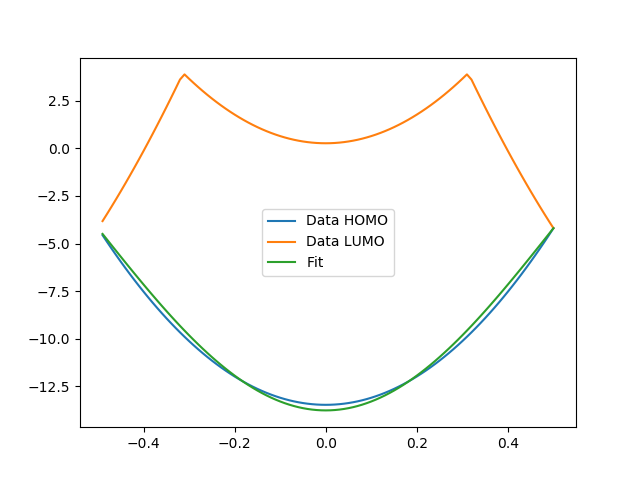
\includegraphics[width = 10cm]{Images/Hydrogen/hydrogen_bandstructure}
	\caption{$E(k)$}
	\label{image_hydrogen_bandstructure}
\end{figure}

In the next step the band structures for the periodically charged hydrogen atoms will be calculated (see \cref{image_hydrogen_charged_bands}). As expected from the symmetry the band structures do not depend on the direction (sign) of the charge displacement. It can also be seen, that the influence of charging is bigger for $k$-points closer to the edge of the Brillouin zone and the bands become shifted to lower energies. Both is in good agreement with the predictions of the Hamiltonian.

\begin{figure}
	\centering
	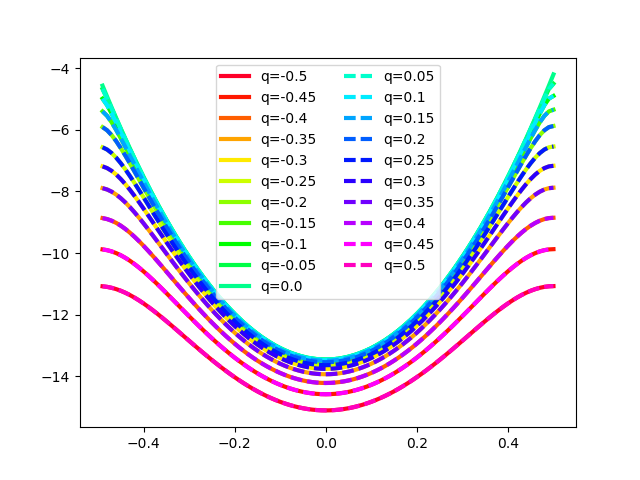
\includegraphics[width = 12cm]{Images/Hydrogen/hydrogen_charged_bands}
	\caption{$E(k, q)$}
	\label{image_hydrogen_charged_bands}
\end{figure}




In \cref{image_hydrogen_charge_potential} the height of the Gaussian potentials causing the charge displacement as a function of the transferred charge is shown. Again the symmetry is as expected and in the region of $-0.2 \le q \le 0.2$ the dependency is approximately linear.

\begin{figure}
	\centering
	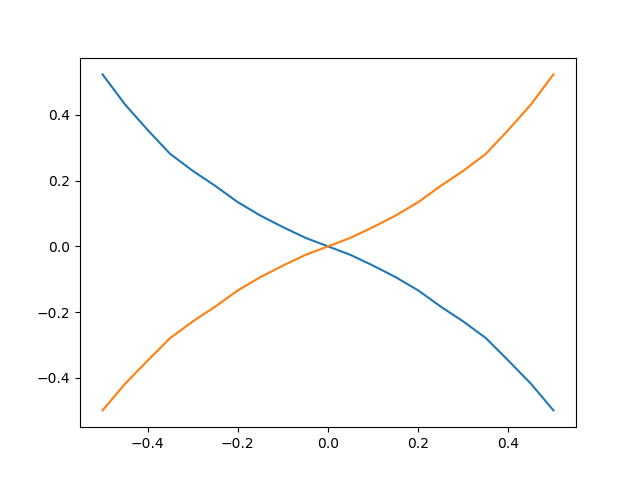
\includegraphics[width = 10cm]{Images/Hydrogen/hydrogen_charge_potential}
	\caption{$V(q)$}
	\label{image_hydrogen_charge_potential}
\end{figure}

From the model Hamiltonian the state energy at the edge of the Brillouin zone ($k\cdot a = \nicefrac{\pi}{2}$) is expected to have the form $E_\text{edge} = -\sqrt{V^2} = -\sqrt{c^2\cdot U_\text{CDFT}^2}$. As can be seen in \cref{image_hydrogen_border_energy_potential} this matches the results of the simulation very well. From a fit to this data the ratio between the theoretical potential and the voltage from CDFT can be obtained: $V \approx \unit[13.265]{e} \cdot U_\text{CDFT}$.

\begin{figure}
	\centering
	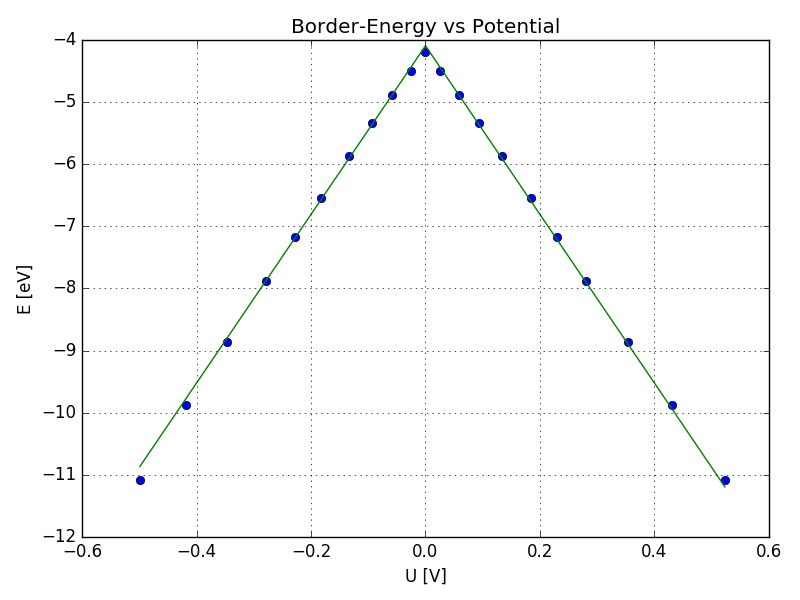
\includegraphics[width = 12cm]{Images/Hydrogen/hydrogen_border_energy}
	\caption{$E(U)$}
	\label{image_hydrogen_border_energy_potential}
\end{figure}

Analogously this ratio can be calculated by fitting the energy at the gamma point to \linebreak $E_\text{gamma} = -\sqrt{c^2 \cdot U_\text{CDFT}^2 + 4 \cdot t_0^2}$ (see \cref{image_hydrogen_mid_energy_potential}). Here the proportionality constant becomes $V \approx \unit[11.289]{e} \cdot U_\text{CDFT}$, which corresponds to a relative difference of approximately 20\%. To take a closer look at this effect the proportionality constant is calculated by fitting for many different $k$-points (see \cref{image_hydrogen_proportionality_constant}). 
\begin{figure}
	\centering
	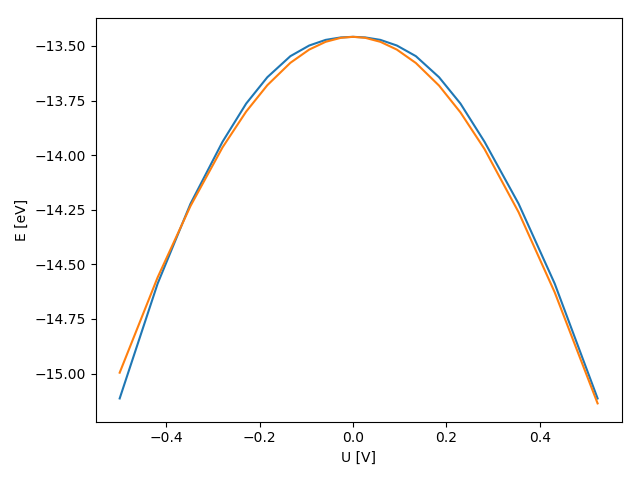
\includegraphics[width = 12cm]{Images/Hydrogen/hydrogen_mid_energy}
	\caption{$E(U)$}
	\label{image_hydrogen_mid_energy_potential}
\end{figure}

\begin{figure}
	\centering
	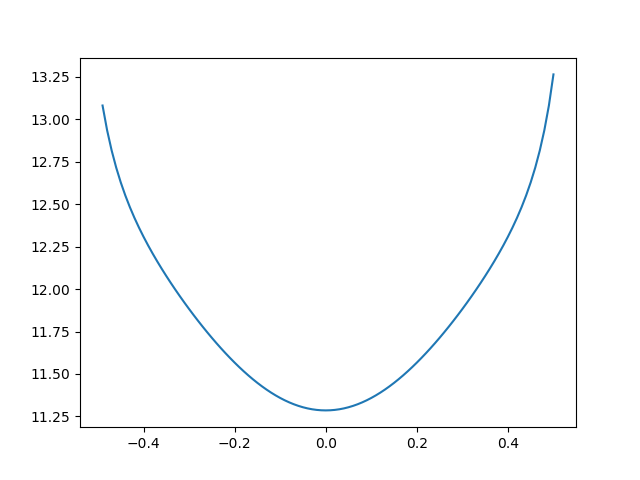
\includegraphics[width = 12cm]{Images/Hydrogen/hydrogen_c_k_dependency}
	\caption{$c(k)$}
	\label{image_hydrogen_proportionality_constant}
\end{figure}